\documentclass[letterpaper,12pt,fleqn]{article}
\usepackage{matharticle}
\usepackage{enumitem}
\pagestyle{plain}
\renewcommand{\o}{\sigma}
\renewcommand{\t}{\tau}
\newcommand{\cycle}[1]{\left<#1\right>}
\begin{document}
Cavallaro, Jeffery \\
Math 221a \\
Homework \#5

\bigskip

\subsection*{1.6.2}
\begin{enumerate}[label={\alph*)}]
\item Prove: $S_n$ is generated by the $(n-1)$ transpositions
  $(12),(13),(14)\ldots,(1n)$.

  Assume $1\le i<j\le n$ \\
  Assume $1\le m\le n$ \\

  $((1i)(1j)(1i))(m)=\begin{cases}
  j, & m=i \\
  i, & m=j \\
  1, & m=1 \\
  m, & m\ne 1\ \mbox{and}\ m\ne i\ \mbox{and}\ m\ne j \\
  \end{cases}$ \\

  $(ij)(m)=\begin{cases}
  j, & m=i \\
  i, & m=j \\
  1, & m=1 \\
  m, & m\ne 1\ \mbox{and}\ m\ne i\ \mbox{and}\ m\ne j \\
  \end{cases}$ \\

  Thus $(1i)(1j)(1i)=(ij)$ \\
  So any transposition $(ij)$ can be generated from the $(n-1)$ transpositions
  $(1x)$ \\
  Assume $\o\in S_n$ \\
  $\o$ can be written as a sequence of disjoint cycles \\
  Each cycle can be written as a sequence of transpositions $(ij)$,
  $1\le i<j\le n$ \\
  Therefore, $\o$ can be generated.

\item Prove: $S_n$ is generated by the $(n-1)$ transpositions
  $(12),(23),(34),\ldots,(n-1\;n)$.

  Assume $1\le i<n$ \\
  Assume $1\le m\le n$ \\

  $((1\;i-1)(i-1\;i)(1\;i-1))(m)=\begin{cases}
  i, & m=1 \\
  1, & m=i \\
  i-1, & m=i-1 \\
  m, & m\ne 1\ \mbox{and}\ m\ne i-1\ \mbox{and}\ m\ne i \\
  \end{cases}$ \\

  $(1i)(m)=\begin{cases}
  i, & m=1 \\
  1, & m=i \\
  i-1, & m=i-1 \\
  m, & m\ne 1\ \mbox{and}\ m\ne i-1\ \mbox{and}\ m\ne i \\
  \end{cases}$ \\

  Thus, $(1\;j-1)(j-1\;j)(1\;j-1)=(1j)$ \\
  So any transposition $(1i)$ can be generated from the (n-1) transpositions
  $(i-1\;i)$ \\
  Therefore, by part (a), any $\o\in S_n$ can be generated.
\end{enumerate}

\subsection*{1.6.3}
Let $\o=(i_1i_2\cdots i_r)\in S_n$ and $\t\in S_n$. \\
Prove: $\t\o\t^{-1}$ is the r-cycle $(\t(i_1)\t(i_2)\cdots\t(i_r))$

Claim: $\t(i_ji_k)\t^{-1}=(\t(i_j)\t(i_k))$ where $0\le j<k\le r$

\begin{description}
\item Case 1: $\t(i_j)=i_j$ and $\t(i_k)=i_k$

  Assume $i_s\ne i_j,i_k$ \\
  $(\t(i_ji_k)\t^{-1})(i_s)=i_s$ \\
  $(\t(i_ji_k)\t^{-1})(i_j)=i_k=\t(i_k)$ \\
  $(\t(i_ji_k)\t^{-1})(i_k)=i_j=\t(i_j)$ \\
  $\therefore \t(i_ji_k)\t^{-1}=(\t(i_j)\t(i_k))$

\item Case 2: $\t^{-1}(i_s)=i_j$ and $\t(i_k)=i_k$ \\
  $i_s=\t(i_j)$ \\
  $(\t(i_ji_k)\t^{-1})(i_s)=\t(i_k)$ \\
  $(\t(i_ji_k)\t^{-1})(\t(i_k))=\t(i_j)$ \\
  $\therefore \t(i_ji_k)\t^{-1}=(\t(i_j)\t(i_k))$

\item Case 3: $\t^{-1}(i_s)=i_j$ and $\t^{-1}(i_t)=i_k$ \\
  $i_s=\t(i_j)$ \\
  $(\t(i_ji_k)\t^{-1})(i_s)=\t(i_k)$ \\
  $(\t(i_ji_k)\t^{-1})(\t(i_k))=\t(i_j)$ \\
  $i_t=\t(i_k)$ \\
  $(\t(i_ji_k)\t^{-1})(i_t)=\t(i_j)$ \\
  $(\t(i_ji_k)\t^{-1})(\t(i_j))=\t(i_k)$ \\
  $\therefore \t(i_ji_k)\t^{-1}=(\t(i_j)\t(i_k))$
\end{description}

$\therefore \t(i_ji_k)\t^{-1}=(\t(i_j)\t(i_k))$

Now:
\begin{eqnarray*}
  \t\o\t^{-1} &=& \t(i_1i_2\cdots i_r)\t^{-1} \\
  &=& \t(i_1i_2)(i_2i_3)\cdots(i_{r-1}i_r)\t^{-1} \\
  &=& \t(i_1i_2)\t^{-1}\t(i_2i_3)\t^{-1}\t\cdots\t^{-1}\t(i_{r-1}i_r)\t^{-1} \\
  &=& (\t(i_1)\t(i_2))(\t(i_2)\t(i_3))\cdots(\t(i_{r-1})\t(i_r)) \\
  &=& (\t(i_1)\t(i_2)\cdots\t(i_r))
\end{eqnarray*}

\subsection*{1.6.3}
\begin{enumerate}[label={\alph*)}]
\item Prove: $S_n=\cycle{(12),(12\cdots n)}$

  Using problem (3):

  $\t(12)\t^{-1}=(\t(1),\t(2))=(23)$ \\
  $\t(23)\t^{-1}=(\t(2),\t(3))=(34)$ \\
  $\vdots$ \\
  $\t(i-1\;i)\t^{-1}=(\t(i-1),\t(i))=(i\;i+1)$ \\
  $\vdots$ \\
  $\t(n-2\;n-1)\t^{-1}=(\t(n-2),\t(n-1))=(n-1\;n)$

  Thus, all possible transpositions of the form $(i-1\;i)$ can be generated,
  and therefore, by problem (2b), all of $S_n$ can be generated.

\item Prove: $S_n=\cycle{(12),(23\cdots n)}$

  Using problem (3):

  $\t(12)\t^{-1}=(\t(1),\t(2))=(13)$ \\
  $\t(13)\t^{-1}=(\t(1),\t(3))=(14)$ \\
  $\vdots$ \\
  $\t(1\;i)\t^{-1}=(\t(1),\t(i))=(1\;i+1)$ \\
  $\vdots$ \\
  $\t(1\;n-1)\t^{-1}=(\t(1),\t(n-1))=(1\;n)$

  Thus, all possible transpositions of the form $(1\;i)$ can be generated,
  and therefore, by problem (2a), all of $S_n$ can be generated.
\end{enumerate}

\subsection*{1.8.1}

Prove that the following are not direct products of their proper subgroups.

In order for a group to be a direct product of its proper subgroups, the
following must hold:
\begin{enumerate}
\item The group must be generated by a collection of its proper, normal,
  almost disjoint subgroups.
\item The group must be isomorphic to the external cross product of those
  subgroups.
\end{enumerate}

\begin{enumerate}[label={\alph*)}]
\item $S_3$

  Although $S_3$ is generated by its 3-element subgroup $\{(),(123),(132)\}$
  and any of its 2-element subgroups, e.g., $\{(),(13)\}$, and although those
  subgroups are almost disjoint, Only the 3-element subgroup is normal; none
  of the 2-element subgroups are normal.

  Moreover, since the 2 and 3 element subgroups are necessarily abelian, their
  external direct product must also be abelian; however, $S_3$ is not abelian
  and thus not isomorphic to the external direct product.

  Therefore $S_3$ is not a direct product of any of its proper subgroups.

\newcommand{\zpn}{\Z_{p^n}}
  
\item $\zpn$

  By Lagrange, all of the proper subgroups of $\zpn$ must be of order $p^k$
  where $1\le k<n$. Since $\zpn$ is abelian, all of its subgroups must also be
  abelian, so all of the proper subgroups are normal. However, we know that
  these subgroups form a chain:
  \[G_p\le G_{p^2}\le\cdots\le G_{p^{n-1}}\]
  Thus, these subgroups are not almost disjoint.
  
  Moreover, all of the elements in all of these subgroups are multiples of
  $p$, in other words $\equiv0\pmod p$. Any other elements are relatively
  prime with $p^n$ and thus are generators of $\zpn$ and are not members of
  any proper subgroup. Thus, elements congruent to $1$ thru $p-1\pmod p$ can
  never be generated by the proper subgroups.

  Therefore $\zpn$ is not the direct product of any of its proper subgroups.

\item $\Z$

  All of the proper subgroups of $\Z$ are the $n\Z$ groups. Since $\Z$ is
  abelian, all of its subgroups must also be abelian, so all of the proper
  subgroups are normal.

  Assume $h\Z$ and $k\Z$ are two such subgroups, $h\ne k$. Then:
  \[hk\in k\Z\]
  \[kh\in h\Z\]
  But since the subgroups are normal:
  \[hk=kh\]
  Thus, $hk\in h\Z\cup k\Z$, so the two subgroups are not almost disjoint.

  Therefore $\Z$ is not the direct product of any of its proper subgroups.
\end{enumerate}

\subsection*{1.8.2}

Given an example of groups $H_i$ and $K_i$ such that
$H_1\times K_1\simeq H_2\times K_2$, and no $H_i$ is isomorphic to any $K_i$.

Consider:
\begin{eqnarray*}
  H_1 &=& \Z_3 \\
  H_2 &=& \Z_4 \\
  K_1 &=& \Z_{20} \\
  H_2 &=& \Z_{15} \\
\end{eqnarray*}
Note that $(3,20)=1$ and $(4,15)=1$, so:
\[H_1\times K_1=\Z_3\times\Z_{20}\simeq\Z_{60}\]
\[H_2\times K_2=\Z_4\times\Z_{15}\simeq\Z_{60}\]
Therefore, $H_1\times K_1\simeq H_2\times K_2$; however, by cardinality, no
$H_i$ is isomorphic to any $K_i$.

\subsection*{1.8.3}

\newcommand{\lr}[2]{\overset{#1}{\underset{#2}\rightleftarrows}}
\newcommand{\rl}[2]{\overset{#1}{\underset{#2}\leftrightarrows}}
\newcommand{\p}{\pi}
\newcommand{\h}{\phi}
\renewcommand{\i}{\iota}
\newcommand{\s}{\psi}
\newcommand{\n}{\mathrel{\triangleleft}}

Let $G$ be additive abelian with subgroups $H$ and $K$. \\
Prove: $G\simeq H\oplus K$ iff there exists homomorphisms
$H\rl{\p_1}{\i_1}G\lr{\p_2}{\i_2}K$ such that:
\begin{eqnarray*}
  \p_1i_1 &=& 1_H \\
  \p_2i_2 &=& 1_K \\
  \p_1i_2 &=& 0 \\
  \p_2i_1 &=& 0 \\
\end{eqnarray*}
and:
\[\forall\,x\in G,(i_1\p_1)(x)+(i_2\p_2)(x)=x\]

\begin{description}
\item $\implies$ Assume $G\simeq H\oplus K$

  Since the direct product holds as defined in the category of groups, we
  have the commutative diagram for the product:

  \begin{tikzpicture}
    \node (G) at (0,3) {$G$};
    \node (K) at (0,0) {$K$};
    \node (H) at (3,3) {$H$};
    \node (HK) at (3,0) {$H\times K$};
    \draw [->] (G) to node [above] {$\p_1$} (H);
    \draw [->] (G) to node [left] {$\p_2$} (K);
    \draw [->] (HK) to node [right] {$\h_1$} (H);
    \draw [->] (HK) to node [below] {$\h_2$} (K);
    \draw [->] (HK) to node [above] {$\h$} (G);
  \end{tikzpicture}

  where the homomorphisms are the canonical projections. Likewise, we have the
  commutative diagram for the co-product:

  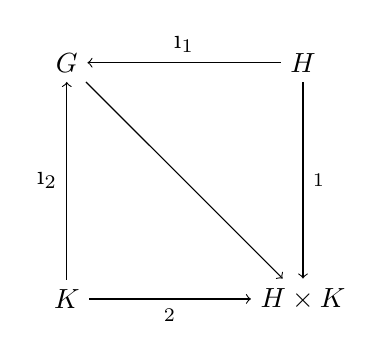
\begin{tikzpicture}
    \node (G) at (0,3) {$G$};
    \node (K) at (0,0) {$K$};
    \node (H) at (3,3) {$H$};
    \node (HK) at (3,0) {$H\times K$};
    \draw [<-] (G) to node [above] {$\i_1$} (H);
    \draw [<-] (G) to node [left] {$\i_2$} (K);
    \draw [<-] (HK) to node [right] {$\s_1$} (H);
    \draw [<-] (HK) to node [below] {$\s_2$} (K);
    \draw [<-] (HK) to node [above] {$\s$} (G);
  \end{tikzpicture}

  where the homomorphisms are the canonical injections.

  Thus, the homomorphisms $H\rl{\p_1}{\i_1}G\lr{\p_2}{\i_2}K$ exist.
  
  Assume $h\in H$:

  $(\p_1\i_1)(h)=\p_1(\i_1(h))=\p_1(h+0)=h$ \\
  $\therefore\p_1\i_1=1_H$

  $(\p_2\i_1)(h)=\p_2(\i_1(h))=\p_2(h+0)=0$ \\
  $\therefore\p_2\i_1=0$

  Assume $k\in K$:
  
  $(\p_2\i_2)(k)=\p_2(\i_2(k))=\p_2(0+k)=k$ \\
  $\therefore\p_2\i_2=1_K$
  
  $(\p_1\i_2)(k)=\p_1(\i_2(k))=\p_1(0+k)=0$
  $\therefore\p_1\i_2=0$

  Assume $x\in G$ \\
  $x=h+k$ for some $h\in H$ and $k\in K$ \\
  \begin{eqnarray*}
    (i_1\p_1)(x)+(i_2\p_2)(x) &=& i_1(\p_1(x))+i_2(\p_2(x)) \\
    &=& i_1(h)+i_2(k) \\
    &=& (h+0)+(0+k) \\
    &=& h+k \\
    &=& x
  \end{eqnarray*}

\item $\impliedby$ Assume all of that other stuff

  Since $H,K\le G$ and $G$ is abelian, $H$ and $K$ are abelian \\
  So, $H\n G$ and $K\n G$ \\
  Thus $H+K\le G$

  Assume $x\in G$ \\
  $x=(i_1\p_1)(x)+(i_2\p_2)(x)=i_1(\p_1(x))+i_2(\p_2(x))$ \\
  Let $\p_1(x)=h\in H$ and $\p_2(x)=k\in K$ \\
  $x=\i_1(h)+i_2(k)=(h+0)+(k+0)=h+k\in H+K$

  Therefore, $H+K=G$

  But, since $\p_1\i_2=0$ and $\p_2\i_1=$, $H$ and $K$ have no projection into
  each other and thus $H\cap K=\{e\}$.

  Therefore, the requirements for corollary 8.7 are met and
  $G\simeq H\oplus K$.
\end{description}
\end{document}
